In the world of crystallography, which encompasses the study of crystals, it can sometimes be nearly impossible to comprehensively describe the structure of a crystal on paper, let alone in words, due to the sheer complexity of these structures. This is why researchers have been using software, which is able to visualise the structure of these crystals, to share their knowledge. Despite the amount of data these programs can already display nowadays, none of them have the full range of 3D virtual reality options current graphic software packages and game engines provide. In this thesis we have focused on one of these in particular, Blender.
\par
Blender is an open source 3D computer graphic software tool which is mainly used for 3D modelling, creating animations and even as a game engine for 3D video games. Blenders makes use of it's own Blender Python API which is, like the software, free to use, and very well documented.
\par
The main goal of this thesis was to firstly see whether it is possible to develop a program in Python that can visualise crystals in Blender. And how this compares to the crystallographic visualisation software which are currently used.
\par
We divided this goal into three general parts: researching the state of the art and programs that might be helpful, actually developing the program and lastly testing the program and analysing the results. 
\par
To get a grasp on the structure of the crystals we want to visualise we explored the world of crystallography. We found that every crystal is build up out of unit cells. A unit cell is a 3D lattice in which the complete structure of a crystal resides. No matter how big a crystal is, it will always consist of a number of these identical unit cells.  
\par
The CIF format is a manner in which crystals can be described with ASCII characters. This makes it interpretable by both humans and computers and made an ideal format to use as input for our program. We used the CifFile module of PyCIFRW to parse these CIF files and convert the crystal data to more usable Python structures.    
\par
The second external program we used is OpenBabel. With OpenBabel we can calculate the positions of all the atoms within the unit cell from a given list of symmetry operation within the crystal. 
\par
To draw the unit cell of a crystal in Blender we needed to make use of the bpy module the Blender API offers. This module contains a lot of functions we used to both create and modify data in the Blender environment. The actual drawing of the crystal consists out of three steps: drawing the frame of the unit cell, drawing the atoms of the unit cell and lastly drawing bonds between atoms. Atoms are drawn as spheres and have different radii and colours based on the element they represent. Whether or not a bond has to be drawn between two atoms, depends on the distance between them. The user has the option to choose this distance or can choose to not draw bonds.
\par
To make our program easy to use, we presented our program in the form of a Blender add-on. Designing an add-on with the Blender API is done by creating a combination of operators classes, which run the functions of the program, and panel classes, with which we can customize the layout of the add-on. 
\par
To test our program we used three crystals with each a different number of atoms, and timed how long it takes for our program to draw these, with and without bonds. We found that for a smaller crystal, this takes about half a second, while for a larger crystal it can take up to two minutes to draw a crystal and its bonds. 
\par
When we compared these results with the time a current crystallographic program, VESTA, takes to draw a crystal, we found that our program takes about 16 times longer to draw a crystal with a small amount of atoms, while it takes up 400 times longer to draw larger crystals. This is mainly due to the fact that the bpy module is rather slow. About 80 percent of the total runtime of our program is used to draw the atoms which means that we only could optimise the remaining 20 percent of the program.
\par
Despite the fact that our program is slower than VESTA, the crystal model it draws is more interactive and the program is both easier to use and more expandable than VESTA. Due to the nearly endless possibilities the combination of the Blender API and Python provide, it is very easy to add features to our program such as the ability to let the user define the boundaries between the crystal has to be drawn and using element specific bonding distances. This makes using Blender as a crystallographic visualisation tool a viable and future proof option and is definitely worth looking into more deeply. 

\begin{figure}[H]
\begin{center}
\begin{tabular}{ll}

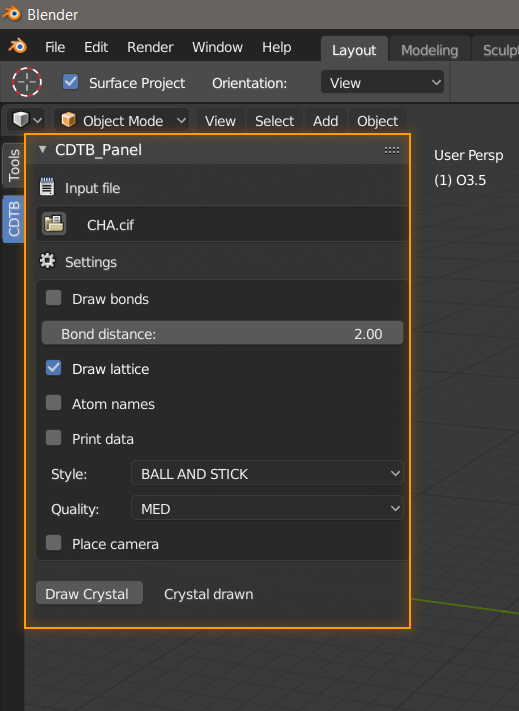
\includegraphics[height=\paperwidth/3]{paneel.png}
&
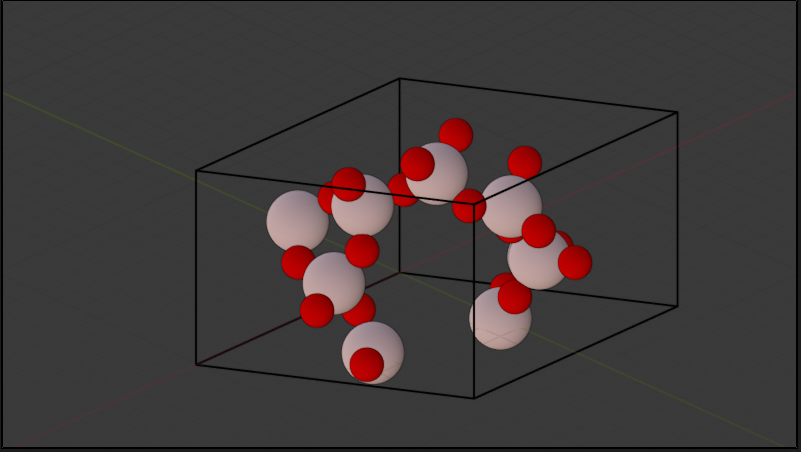
\includegraphics[width=\paperwidth/3]{OSO_max.png}

\end{tabular}
\end{center}
\end{figure}